\chapter{From Power Plant to Home: The Alternator}\label{ch:g9:alternator}

A year's worth of \omterm{def:g9:electric-power-energy:kwh}{kilowatt-hours} has flowed through your
audits --- but from where? Follow the cable out of the house,
under the street, across the pylons, and it ends at a machine
spinning in a great hall: the \omterm{def:g9:alternator:alternator}{alternator}. Its secret is the
loveliest surprise in this book's electricity: the
current-makes-magnetism discovery of last year, run backward.

\section{Induction: the effect reversed}

\begin{proposition}[Electromagnetic induction]\label{prop:g9:alternator:induction}
Move a \omterm{def:g1:magnets:magnet}{magnet} near a \omterm{def:g3:first-electric-circuit:circuit}{closed circuit} --- or move the circuit
near the \omterm{def:g1:magnets:magnet}{magnet} --- and while the motion lasts, a \omterm{def:g8:voltage-voltmeter:voltage}{voltage}
appears and drives a current: electricity \emph{induced} by
changing magnetism. The rules, from the bench:
\begin{enumerate}
  \item only \emph{change} induces: \omterm{def:g1:magnets:magnet}{magnet} at rest beside the
        coil, nothing --- however strong the \omterm{def:g1:magnets:magnet}{magnet};
  \item faster motion, stronger \omterm{def:g1:magnets:magnet}{magnet}, more turns of coil:
        bigger induced \omterm{def:g8:voltage-voltmeter:voltage}{voltage};
  \item reverse the motion, reverse the induced current ---
        approach and retreat drive opposite marches.
\end{enumerate}
Last year a current made magnetism; this year moving
magnetism makes a current. The two effects are one coin,
read from its two faces --- and the second face \omterm{def:g9:electric-power-energy:power}{powers}
civilization.
\end{proposition}

\begin{method}[Induction on the bench]\label{met:g9:alternator:bench}
A coil of many turns, a bar \omterm{def:g1:magnets:magnet}{magnet}, a sensitive
zero-centered meter:
\begin{enumerate}
  \item connect the meter across the coil; hold the \omterm{def:g1:magnets:magnet}{magnet}
        still inside it: the needle sleeps at zero ---
        strength alone induces nothing;
  \item thrust the \omterm{def:g1:magnets:magnet}{magnet} in: the needle kicks one way ---
        and returns to zero the instant the motion stops;
  \item withdraw it: an equal kick, the other way;
  \item thrust faster: a bigger kick. Jiggle the \omterm{def:g1:magnets:magnet}{magnet} in
        and out rhythmically, and the needle swings left,
        right, left --- you are hand-cranking an \omterm{def:g9:alternating-current:dcac}{alternating
        current}.
\end{enumerate}
\end{method}

\begin{omfigure}
\begin{tikzpicture}[scale=0.85]
  \draw[thick, fill=omThm, fill opacity=0.5]
    (0.4,1.2) rectangle (2.6,2.0);
  \node[font=\small] at (1.5,1.6) {N \quad S};
  \draw[-Stealth, very thick, omExo] (2.9,1.6) -- (4.0,1.6);
  \foreach \x in {4.4,4.8,...,6.8} {
    \draw[very thick, omDef] (\x,0.9) arc (200:340:0.32 and 0.75);
  }
  \draw[thick, omDef] (4.4,0.9) -- (4.1,0.2);
  \draw[thick, omDef] (7.4,0.9) -- (7.7,0.2);
  \draw[thick] (4.1,0.2) -- (4.1,-0.4) -- (5.2,-0.4);
  \draw[thick] (7.7,0.2) -- (7.7,-0.4) -- (6.1,-0.4);
  \draw[thick, fill=white] (5.65,-0.4) circle (0.45);
  \draw[-Stealth, very thick, omThm] (5.65,-0.4) -- ++(60:0.38);
  \node[right, font=\small] at (7.9,1.6)
    {thrust the magnet: the needle kicks};
  \node[right, font=\small] at (7.9,1.0)
    {hold it still: the needle sleeps};
\end{tikzpicture}

{\small Induction on the bench: only a \emph{moving} \omterm{def:g1:magnets:magnet}{magnet}
wakes the coil --- and the needle's kick reverses with the
motion.}
\end{omfigure}

\section{The alternator}

\begin{definition}[Alternator]\label{def:g9:alternator:alternator}
An \emph{alternator}\index{alternator} is induction made
tireless: a \omterm{def:g1:magnets:magnet}{magnet} spun steadily beside a fixed coil (or a
coil spun in a magnetic field). Each half-turn brings a pole
toward the coil, then carries it away --- change, endlessly
renewed --- so the induced \omterm{def:g8:voltage-voltmeter:voltage}{voltage} swings positive, negative,
positive: \emph{alternating}, by construction, tracing
exactly the smooth sinusoid of the \omterm{met:g9:alternating-current:scope}{oscilloscope} chapter. Spin
at fifty turns a second and the output alternates at
\qty{50}{Hz}: the grid's \omterm{def:g8:sound-pitch-loudness:frequency}{frequency} \emph{is} a rotation
\omterm{def:g7:motion-average-speed:formula}{speed}, kept in lockstep by every station on the network.
\end{definition}

\begin{example}[The dynamo on your wheel]\label{ex:g9:alternator:dynamo}
The bicycle dynamo is a pocket \omterm{def:g9:alternator:alternator}{alternator}: the wheel spins a
little \omterm{def:g1:magnets:magnet}{magnet} inside a fixed coil, and the lamp \omterm{def:g1:light-and-shadows:source}{lights} ---
brighter and at higher \omterm{def:g8:sound-pitch-loudness:frequency}{frequency} as you pedal harder, exactly
as the bench rules promise (and flickering at a crawl, as the
alternating chapter observed). Its price is honest too: the
dynamo drags --- lighting the lamp costs your legs real
effort. Induction gives no \omterm{def:g5:everyday-energy:energy}{energy}; it \emph{converts} motion
into electricity, \omterm{def:g9:kinetic-energy-safety:joule}{joule} for \omterm{def:g9:kinetic-energy-safety:joule}{joule}, minus friction's tax.
\end{example}

\begin{omfigure}
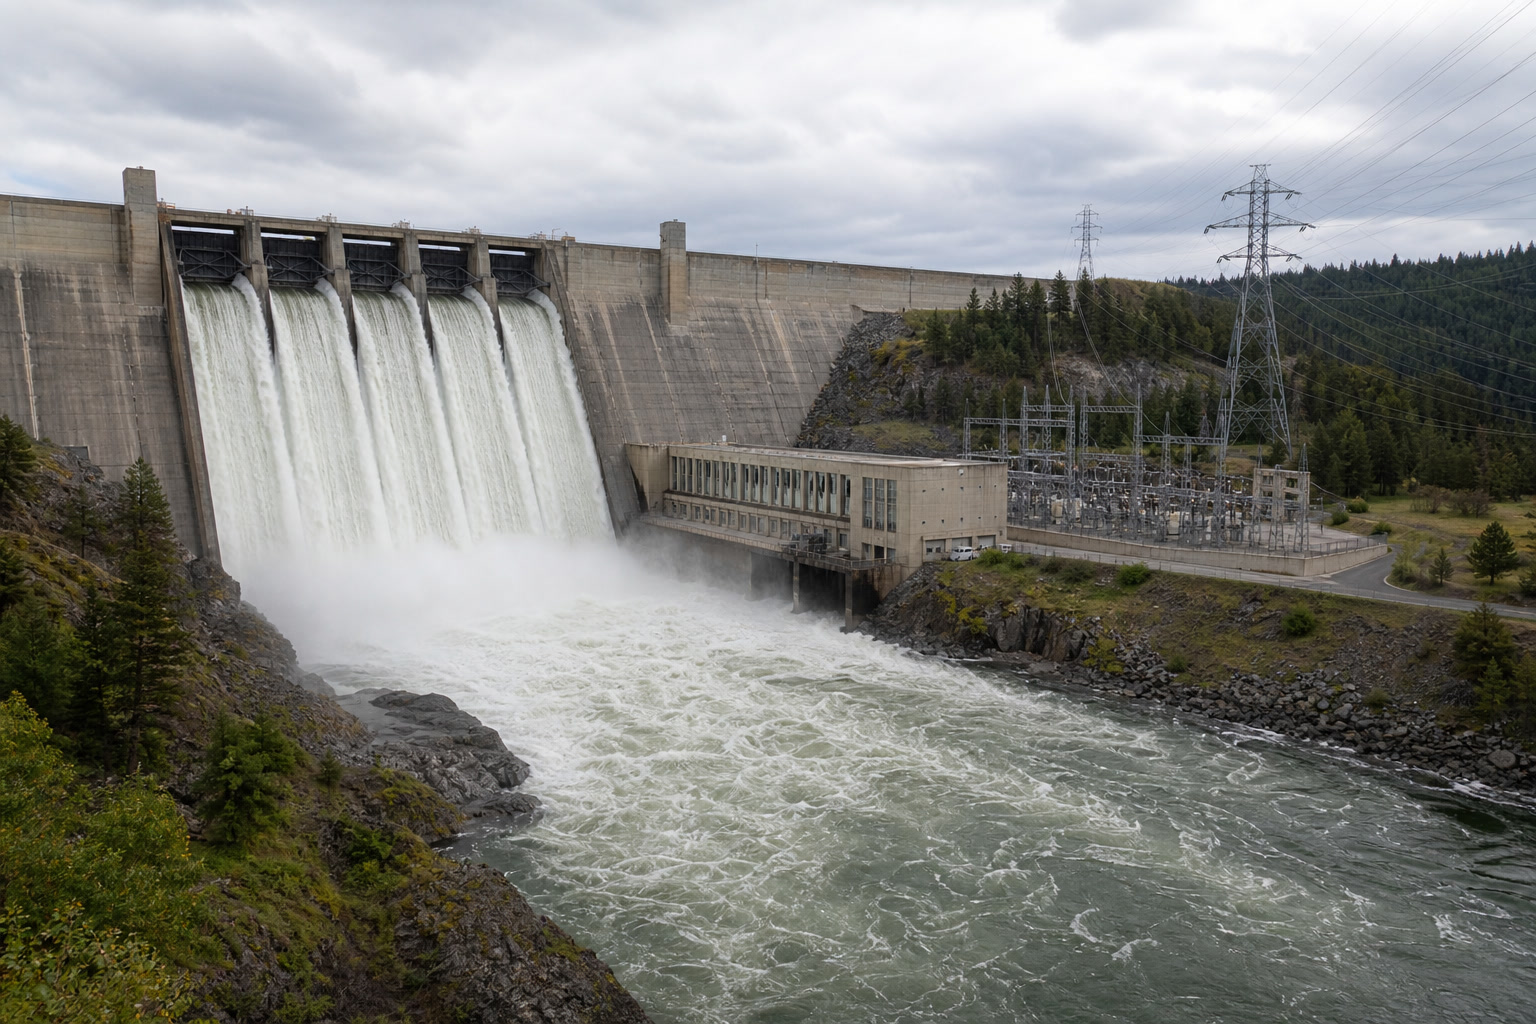
\includegraphics[width=0.55\linewidth]{images/book1/ai/g9-alternator-dam.jpg}

{\small A hydroelectric plant: lifted water rushes down, spins the turbines, and the \omterm{def:g9:alternator:alternator}{alternators} send the \omterm{def:g5:everyday-energy:energy}{energy} away along the wires.}
\end{omfigure}

\section{Every power plant is one machine}

\begin{proposition}[The common core]\label{prop:g9:alternator:core}
Nearly all the world's electricity, whatever its
advertisement, is made the same way: something spins a
\emph{turbine} --- a sturdy windmill of blades --- and the
turbine spins an \omterm{def:g9:alternator:alternator}{alternator}. \omterm{def:g9:electric-power-energy:power}{Power} plants differ only in
\emph{what pushes the blades}:
\begin{enumerate}
  \item thermal plants boil water with burning coal or gas
        --- steam jets drive the turbine;
  \item nuclear plants boil the water instead with the
        \omterm{def:g5:heat-and-insulation:heat}{heat} of splitting atoms --- steam again;
  \item hydroelectric dams let a mountain lake fall through
        the blades --- the childhood dam-chain, completed;
  \item \omterm{def:g2:air-around-us:wind}{wind} turbines skip the middleman: the \omterm{def:g2:air-around-us:wind}{wind} is the
        blades' push, an \omterm{def:g9:alternator:alternator}{alternator} in every nacelle.
\end{enumerate}
One exception proves the rule: solar panels make electricity
with no spin at all --- by a \omterm{def:g1:light-and-shadows:source}{light} effect belonging to the
university years.
\end{proposition}

\begin{omfigure}
\begin{tikzpicture}[scale=0.8]
  \node[draw, thick, omExo, font=\footnotesize, align=center,
    minimum width=2.1cm, minimum height=0.95cm] (src) at (0.9,0)
    {flame, atom,\\lake or wind};
  \node[draw, thick, omMeth, font=\footnotesize, align=center,
    minimum width=1.9cm, minimum height=0.95cm] (tur) at (3.8,0)
    {turbine\\(spin!)};
  \node[draw, thick, omThm, font=\footnotesize, align=center,
    minimum width=2.0cm, minimum height=0.95cm] (alt) at (6.6,0)
    {alternator\\(induction)};
  \node[draw, thick, omDef, font=\footnotesize, align=center,
    minimum width=2.0cm, minimum height=0.95cm] (gri) at (9.5,0)
    {transformer\\and grid};
  \draw[-Stealth, very thick] (src) -- (tur);
  \draw[-Stealth, very thick] (tur) -- (alt);
  \draw[-Stealth, very thick] (alt) -- (gri);
  \node[below, font=\footnotesize] at (2.35,-0.75) {heat or motion};
  \node[below, font=\footnotesize] at (5.2,-0.75) {rotation};
  \node[below, font=\footnotesize] at (8.05,-0.75)
    {alternating current};
\end{tikzpicture}

{\small Every plant, one chain: something spins the turbine,
the turbine spins the \omterm{def:g9:alternator:alternator}{alternator}, and induction does the
rest. Only the first box differs from plant to plant.}
\end{omfigure}

\begin{example}[Chains, audited]\label{ex:g9:alternator:chains}
Write each plant as a childhood \omterm{def:g5:everyday-energy:energy}{energy} chain, now with
professional vocabulary. The dam: stored height $\to$ motion
of falling water $\to$ rotation $\to$ electricity --- the
Sun, remember, lifted that lake by evaporation: hydro \omterm{def:g9:electric-power-energy:power}{power}
is rain-deferred sunshine. The coal plant: chemical store
$\to$ \omterm{def:g5:heat-and-insulation:heat}{heat} $\to$ steam's motion $\to$ rotation $\to$
electricity --- with warmth leaking at every arrow, as the
cooling towers' plumes confess. \omterm{def:g2:air-around-us:wind}{Wind}: moving \omterm{def:g2:air-around-us:air}{air} (stirred by
the Sun) straight to rotation. Sources that nature refills
--- water, \omterm{def:g2:air-around-us:wind}{wind}, sunlight --- are called
\emph{renewable}\index{renewable}; the burned and split
stores are spent forever on human timescales.
\end{example}

\begin{remark}[Why the pylons hum at 400000 volts]\label{rem:g9:alternator:transport}
The last promise of the alternating chapter falls due. A
town needs, say, a hundred million \omterm{def:g9:electric-power-energy:power}{watts}. By $P = U I$, that
\omterm{def:g9:electric-power-energy:power}{power} can travel as an enormous current at modest \omterm{def:g8:voltage-voltmeter:voltage}{voltage}
--- or a modest current at enormous \omterm{def:g8:voltage-voltmeter:voltage}{voltage}. But wires \omterm{def:g5:heat-and-insulation:heat}{heat}
with the \emph{current} (the old \omterm{prop:g8:electric-current-effects:three}{heating effect}), and every
degree of pylon-warming is paid-for \omterm{def:g5:everyday-energy:energy}{energy} lost to the
crows. So the grid transports at breathtaking \omterm{def:g8:voltage-voltmeter:voltage}{voltages} ---
hundreds of thousands of \omterm{def:g8:voltage-voltmeter:voltage}{volts}, tiny currents, minimal loss
--- and steps the \omterm{def:g8:voltage-voltmeter:voltage}{voltage} down, neighborhood by
neighborhood, to the tame \qty{230}{V} of your wall. The
stepping machine, the \emph{transformer}, is two coils and
induction once more --- and it works only on current that
alternates: the whole grid speaks AC because the
transformer does.
\end{remark}

\section{Exercises}

\begin{exercise}[$\star$]\label{exo:g9:alternator:1}
State the three bench rules of induction. What does a
strong \omterm{def:g1:magnets:magnet}{magnet} \emph{at rest} induce?
\end{exercise}

\begin{exercise}[$\star$]\label{exo:g9:alternator:2}
Why does an \omterm{def:g9:alternator:alternator}{alternator}'s output alternate? Tie the sign
changes to the rotation.
\end{exercise}

\begin{exercise}[$\star$]\label{exo:g9:alternator:3}
At what rotation \omterm{def:g7:motion-average-speed:formula}{speed} does an \omterm{def:g9:alternator:alternator}{alternator} feed a
\qty{50}{Hz} grid? What must every station on the network
therefore agree on?
\end{exercise}

\begin{exercise}[$\star$]\label{exo:g9:alternator:4}
Name the two universal boxes of every power plant, and the
one box that changes between coal, atom, dam and \omterm{def:g2:air-around-us:wind}{wind}.
\end{exercise}

\begin{exercise}[$\star$]\label{exo:g9:alternator:5}
Write the hydroelectric chain from mountain lake to your
lamp --- and name the celestial machine that filled the
lake.
\end{exercise}

\begin{exercise}[$\star$]\label{exo:g9:alternator:6}
Why does pedaling grow harder the instant the dynamo's lamp
switches on? Which principle forbids it being otherwise?
\end{exercise}

\begin{exercise}[$\star$]\label{exo:g9:alternator:7}
Sort into \omterm{ex:g9:alternator:chains}{renewable} and not: \omterm{def:g2:air-around-us:wind}{wind}; coal; the dam's lake;
uranium; sunlight. What defines the sorting?
\end{exercise}

\begin{exercise}[$\star$]\label{exo:g9:alternator:8}
Why does the grid ship its \omterm{def:g9:electric-power-energy:power}{power} at hundreds of thousands
of \omterm{def:g8:voltage-voltmeter:voltage}{volts}? Name the formula that offers the choice and the
effect that decides it.
\end{exercise}

\begin{exercise}[$\star\star$]\label{exo:g9:alternator:9}
A demonstration \omterm{def:g9:alternator:alternator}{alternator} hand-cranked slowly \omterm{def:g1:light-and-shadows:source}{lights} its
lamp faintly with visible flicker; cranked fast, brightly
and steadily. Account for both changes with the bench rules
and the \omterm{def:g8:sound-pitch-loudness:frequency}{frequency} chapter.
\end{exercise}

\begin{exercise}[$\star\star$]\label{exo:g9:alternator:10}
A plant delivers \qty{1e8}{W}. Compare the currents needed
at \qty{230}{V} and at \qty{400000}{V} (scientific
notation). Which could real cables carry?
\end{exercise}

\begin{exercise}[$\star\star$]\label{exo:g9:alternator:11}
Thermal and nuclear plants are, at heart, elaborate
kettles. Defend this slogan with their chains --- and
locate the one link where the two differ.
\end{exercise}

\begin{exercise}[$\star\star\star$]\label{exo:g9:alternator:12}
The grand tour, run backward: tonight your lamp glows at
\qty{230}{V}. Trace its \omterm{def:g5:everyday-energy:energy}{energy} upstream through every box
--- transformer, pylons, \omterm{def:g9:alternator:alternator}{alternator}, turbine, and one
primary store of your choosing --- naming the \omterm{def:g5:everyday-energy:energy}{energy}
form at each stage and the leaks along the way. Then
answer the childhood question with a year-nine sentence:
where does the \omterm{def:g1:light-and-shadows:source}{light} in your room ultimately come from?
\end{exercise}

\section{Problem: Night Shift at the Station}

\begin{problem}[{Weekend problem --- night shift at the
hydroelectric station; induction, lockstep and the storm;
the engineer's log}]\label{pb:g9:alternator:1}
You \omterm{def:g1:light-and-shadows:shadow}{shadow} the night engineer at the valley's dam --- lake
above, town below, \omterm{def:g9:alternator:alternator}{alternators} humming between.

\medskip\noindent\textbf{Part I --- The machine hall.}
\begin{enumerate}
  \item The engineer opens a gate: water thunders through
        turbine three, and its \omterm{def:g9:alternator:alternator}{alternator}'s meters wake.
        Write the \omterm{def:g5:everyday-energy:energy}{energy} chain from lake to busbar.
  \item Inside the \omterm{def:g9:alternator:alternator}{alternator}, what moves and what stands
        still --- and why must something move at all?
  \item The grid runs at \qty{50}{Hz}. The engineer
        watches a dial keeping turbine three at exactly
        the matching rotation. What goes wrong at the
        wrong \omterm{def:g7:motion-average-speed:formula}{speed}? (What would its \omterm{def:g8:voltage-voltmeter:voltage}{voltage}'s \omterm{def:g8:sound-pitch-loudness:frequency}{frequency}
        do?)
  \item A trainee asks whether a stronger \omterm{def:g1:magnets:magnet}{magnet} in the
        rotor would give ``free'' extra \omterm{def:g9:electric-power-energy:power}{power}. Correct the
        dream with the dynamo's honest price.
\end{enumerate}

\medskip\noindent\textbf{Part II --- The town's demand.}
\begin{enumerate}[resume]
  \item At 03:00 the town draws \qty{2e7}{W}. At
        the transport line's \qty{200000}{V}, what current
        leaves the station?
  \item The same \omterm{def:g9:electric-power-energy:power}{power} at \qty{230}{V} would need what
        current --- and what does the comparison say about
        the transformer's job?
  \item At 07:00, kettles and heaters wake:
        demand doubles. What must the engineer feed the
        turbines more of, and what would happen to the
        grid's \omterm{def:g8:sound-pitch-loudness:frequency}{frequency} if she fed too little? (The
        machines slow under load, like a cyclist on a
        hill.)
  \item The station's sister plant --- a \omterm{def:g2:air-around-us:wind}{wind} farm on the
        ridge --- drops out as the \omterm{def:g2:air-around-us:wind}{wind} dies. Which box of
        its chain failed, and which boxes stood entirely
        healthy?
\end{enumerate}

\medskip\noindent\textbf{Part III --- The storm.}
\begin{enumerate}[resume]
  \item Lightning severs a transport line; breakers fire.
        The engineer reroutes \omterm{def:g9:electric-power-energy:power}{power} along neighboring
        lines. What property of the grid --- one great
        parallel network --- makes rerouting possible?
  \item During the scramble, a warehouse's \omterm{def:g1:light-and-shadows:source}{lights} dim
        brown for a minute. Interpret: what sagged, and
        what were the warehouse's \omterm{ex:g6:circuits-and-safety:motor}{motors} and lamps briefly
        underfed?
  \item Dawn: the log must explain to the trainees why
        the whole night's electricity was, at origin,
        sunshine. Draft the two-line explanation (lake,
        evaporation, rain).
  \item Final line of the log, by tradition: the night's
        physics in one sentence --- motion, magnetism,
        and the town's morning kettle in it.
\end{enumerate}
\end{problem}
